% !TeX root = ../thesis_main.tex

% ---------------------------------------------------
% ----- Chapters of the template
% ----- for Bachelor-, Master thesis and class papers
% ---------------------------------------------------
%  Created by C. Müller-Birn on 2012-08-17, CC-BY-SA 3.0.
%  Freie Universität Berlin, Institute of Computer Science, Human Centered Computing. 
%
\chapter{Prototyping}
\label{chap:prototyping} 

After collecting the initial user feedback, digital ``paper'' prototypes were created using Figma\footnote{Figma (\url{https://www.figma.com/}) is a design tool accessible through the browser for collaborative work on design projects.} to gather visualizations of possible UI layouts.
Two ideas emerged from the interviews: a (file-)editor-centric layout and a preview-centric layout.
\section{Editor centric vs. preview centric layout}

The \textbf{preview-centric layout} is inspired by popular generic website builders like \url{https://wix.com} or \url{https://wordpress.com} / Elementor.
A preview-centric UI editor, also referred to as WYSIWYG (what you see is what you get) editor, lets the user directly interact with a preview of the final layout.
Often this means composing ``elements'' or ``blocks'' per drag and drop (1 and 2 in fig. \ref{fig:preview-centric}), and when a component is selected, additional options of this component can be configured (3 in fig. \ref{fig:preview-centric}).
This approach requires little cognitive transfer from the user, since the preview is at the same time the source of truth of the configuration.
On the other hand, this WYSIWYG approach is impractical when a lot of the data and parts of the UI are dynamically loaded and dependent on user state.
For example, a common use case for Purple apps is to show special offers only on one platform or to hide components for users who are not logged in.
Discovering and configuring these invisible elements can lead to confusion by the users. 
\begin{figure}[h!]
  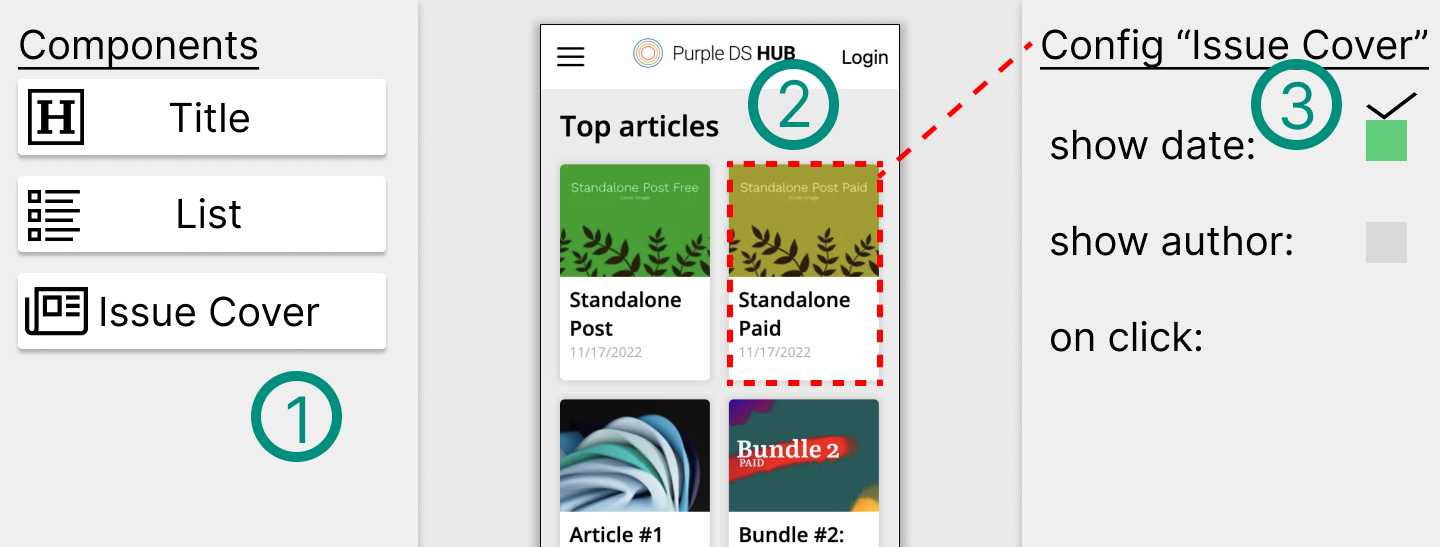
\includegraphics[width=\textwidth]{pics/preview_centric.png}
  \caption[Preview-centric prototype]{Preview-centric prototype from figma. Labels: \textit{1}: component library, \textit{2}: preview, \textit{3}: options for selected component}
  \label{fig:preview-centric}
\end{figure}
\newpage
The \textbf{editor-centric layout} is inspired by modern text editors / \Gls{ide}s like VS Code (\url{https://code.visualstudio.com/}), which was mentioned as reference during the interviews multiple times.
In this approach, the underlying configuration structure is more visible to the user, which is often done via text files.
The central pane is the editor for the currently open file, while on the sides additional panes for file management and selection, preview and more can be shown.
The familiarity, especially to developers who are used to IDE layouts, could help new users adopt patterns to work with the UI they use in other tools as well.
\begin{figure}[h!]
  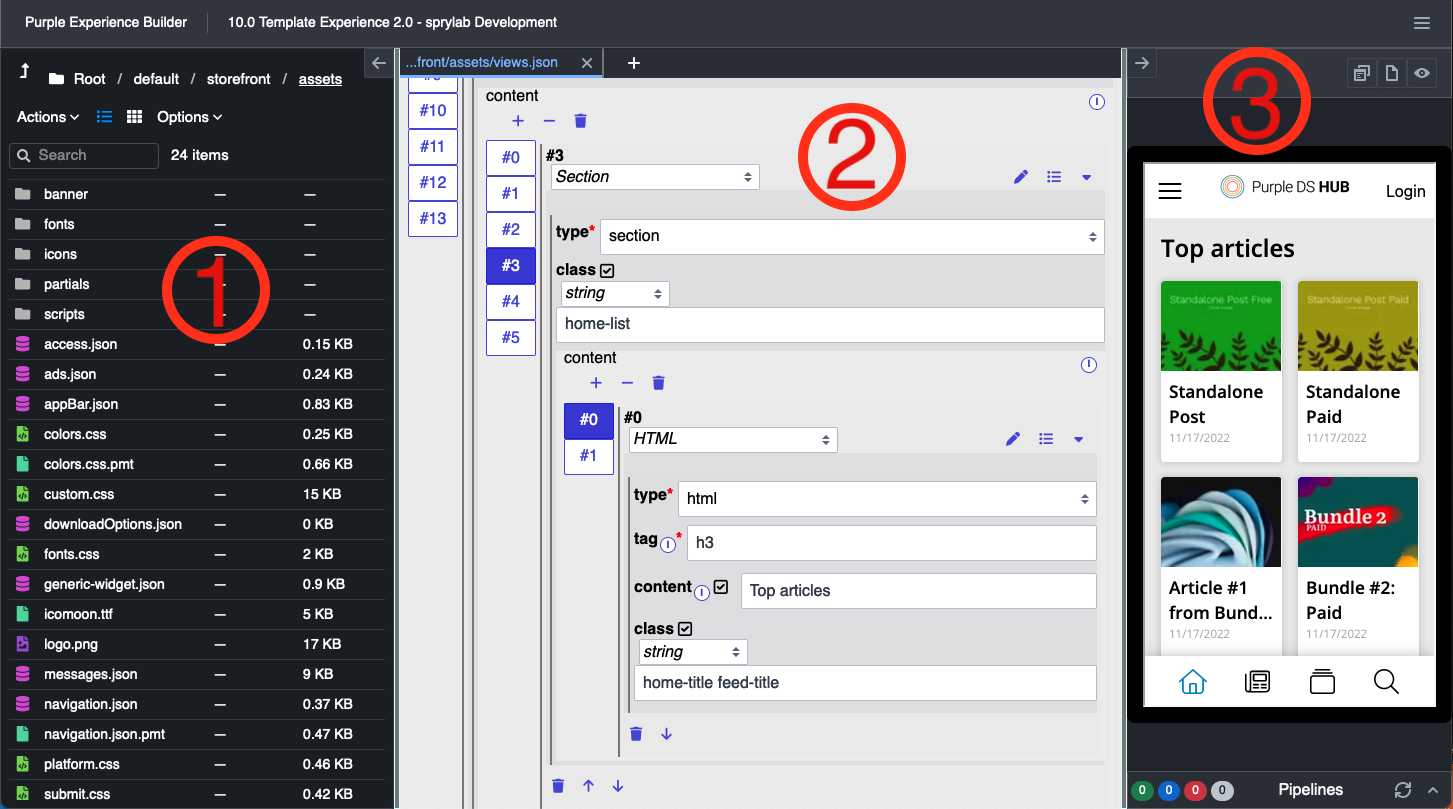
\includegraphics[width=\textwidth]{pics/editor-centric-screenshot.png}
  \caption{Editor centric todo}
  \label{fig:editor-centric}
\end{figure}
\bigskip

For the UI editor, the choice fell on the editor-centric approach, for which the reasons are explained below.
\begin{itemize}
  \item Existing libraries / tools like \url{https://vwo.com/why-us/technology/visual-editor/} or WordPress Elementor are not adaptable enough to fit into the configuration structure of the  \Gls{experience}. It was not built with preview-based editing in mind, so the already mentioned problems of invisible or platform dependent UI components is decisive.
  \item Implementing a custom preview-centric solution seems more complicated and uncertain to result in a viable product within the limited time frame of this thesis. For editor-centric UIs, many third-party libraries exist that can be integrated, such as Microsoft's Monaco Editor (\url{https://microsoft.github.io/monaco-editor/}) with automatic syntax highlighting for a wide range of file types.
  \item The user base consists mostly of tech-affine people who are used to layouts of IDEs. As Jakob's Law of the Internet User Experience states, the user's understanding of a website is directly tied to their mental model of that system \cite{Nielsen:2000} and \cite[p. 2]{LawsOfUX:2020ys}. Introducing an unconventional workflow comes with the danger of confusing the user, causing mistakes, and potentially leading to dissatisfaction with the tool.
\end{itemize}

